\chapter{Primer anexo}
Este capítulo (anexo) es opcional, y se escribirá de acuerdo con las indicaciones del Tutor.

\begin{figure}[h]
	\centering
	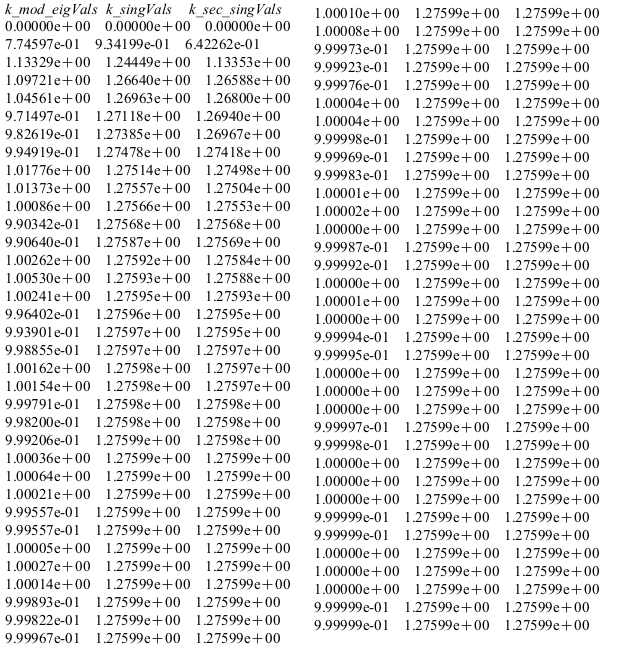
\includegraphics[width=0.8\textwidth]{include/a-1b1t2t10_traza.png}
	\caption{Ejemplo 1.}
	\label{fig:a-1b1t2t10_traza}
\end{figure}

\begin{figure}[h]
	\centering
	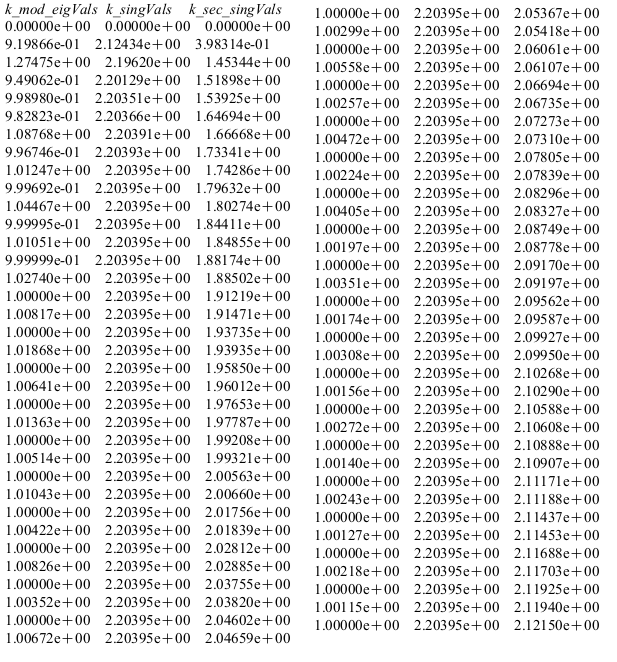
\includegraphics[width=0.8\textwidth]{include/a-1b1t10t2_traza.png}
	\caption{Ejemplo 2.}
	\label{fig:a-1b1t10t2_traza}
\end{figure}

\begin{figure}[h]
	\centering
	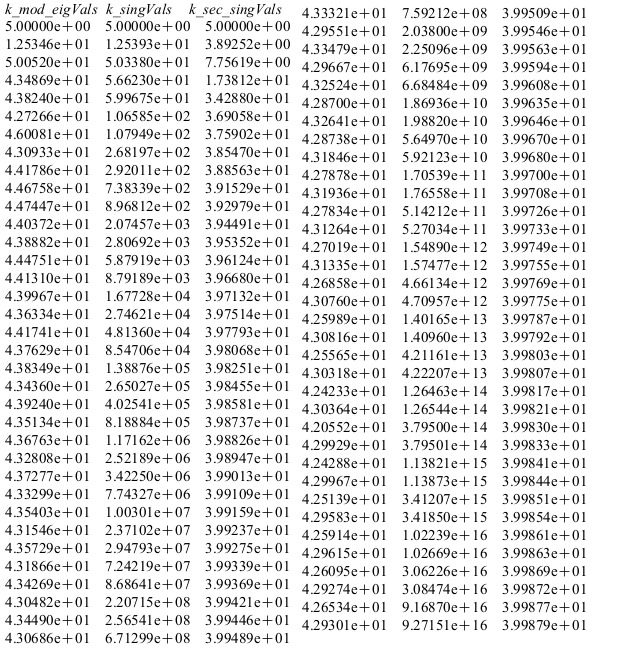
\includegraphics[width=0.8\textwidth]{include/a0b10c30d40_traza.png}
	\caption{Ejemplo 3.}
	\label{fig:a0b10c30d40_traza}
\end{figure}

\begin{figure}[h]
	\centering
	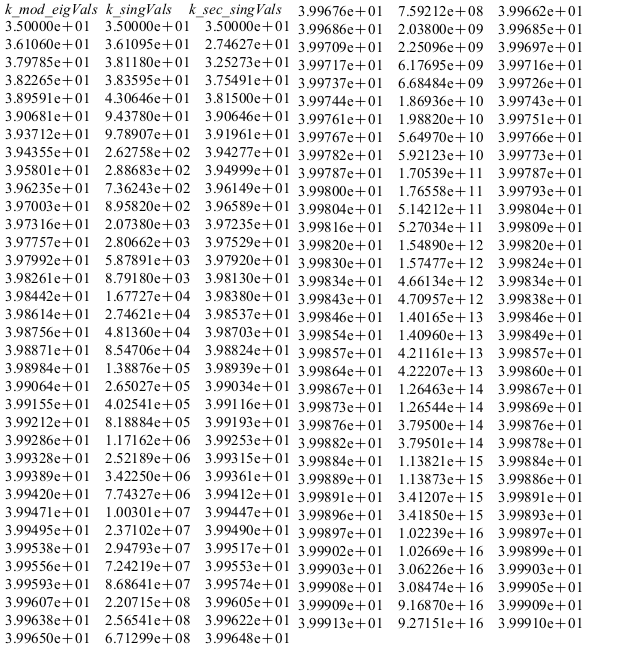
\includegraphics[width=0.8\textwidth]{include/a30b40c0d10_traza.png}
	\caption{Ejemplo 4.}
	\label{fig:a30b40c0d10_traza}
\end{figure}

\begin{figure}[h]
	\centering
	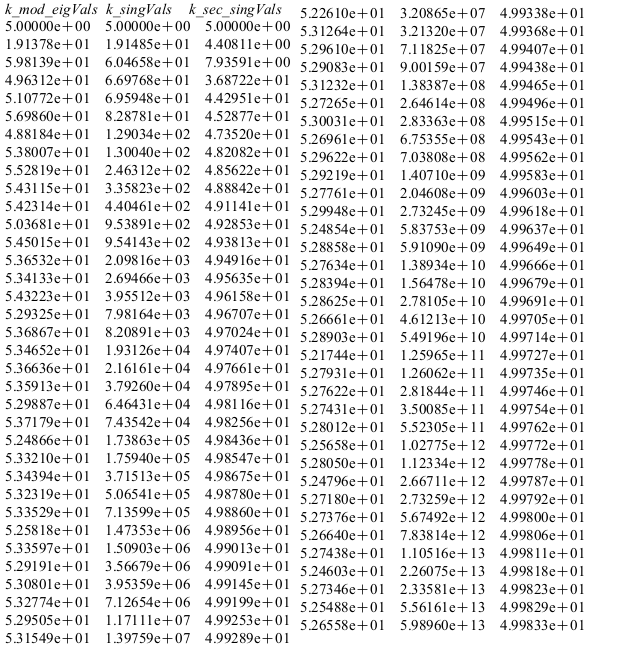
\includegraphics[width=0.8\textwidth]{include/a0b10c30d50_traza.png}
	\caption{Ejemplo 5.}
	\label{fig:a0b10c30d50_traza}
\end{figure}

\begin{figure}[h]
	\centering
	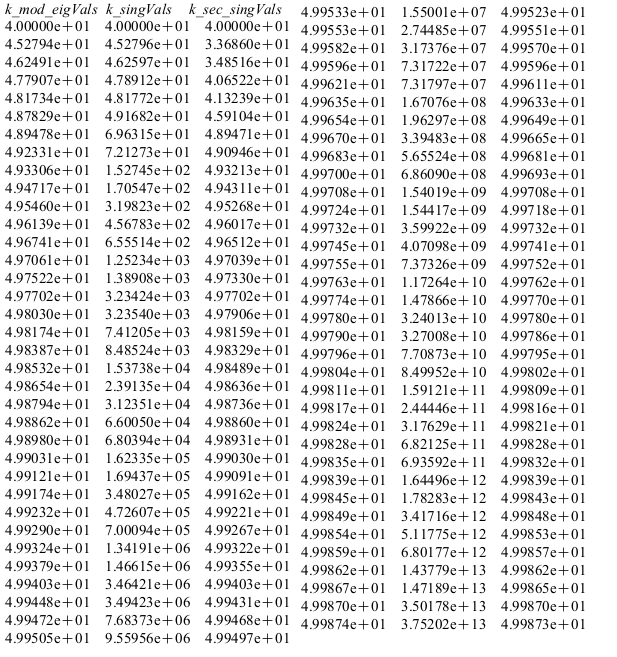
\includegraphics[width=0.8\textwidth]{include/a30b50c0d10_traza.png}
	\caption{Ejemplo 6.}
	\label{fig:a30b50c0d10_traza}
\end{figure}

\begin{figure}[h]
	\centering
	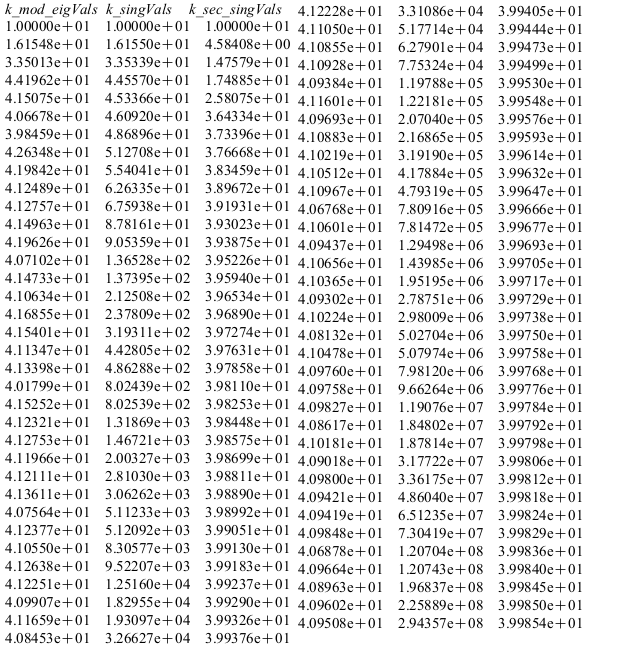
\includegraphics[width=0.8\textwidth]{include/a0b20c30d40_traza.png}
	\caption{Ejemplo 7.}
	\label{fig:a0b20c30d40_traza}
\end{figure}

\begin{figure}[h]
	\centering
	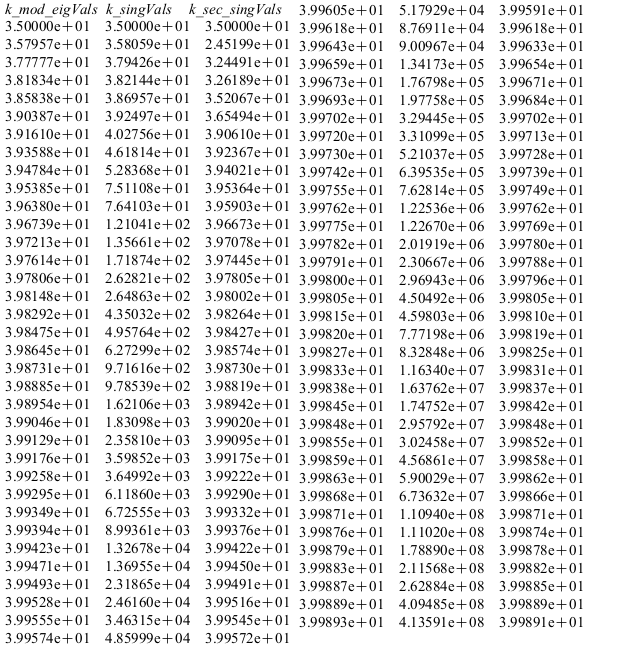
\includegraphics[width=0.8\textwidth]{include/a30b40c0d20_traza.png}
	\caption{Ejemplo 8.}
	\label{fig:a30b40c0d20_traza}
\end{figure}

\begin{figure}[h]
	\centering
	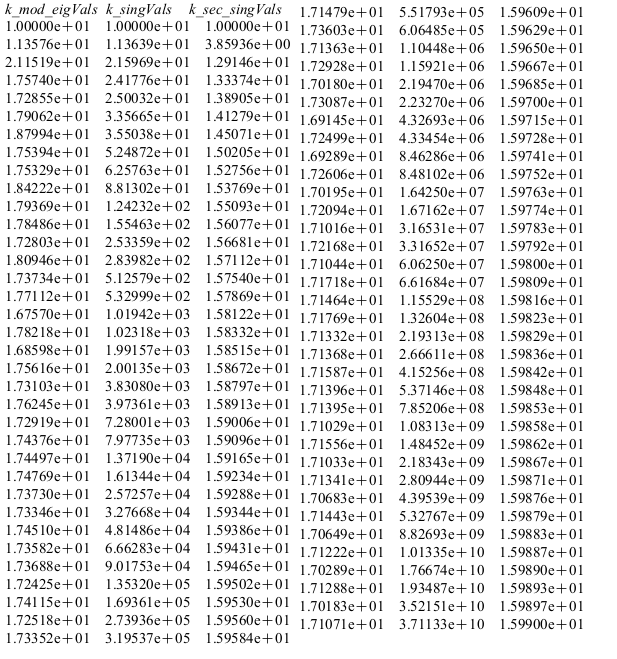
\includegraphics[width=0.8\textwidth]{include/a-15b-5c5d16_traza.png}
	\caption{Ejemplo 8.}
	\label{fig:a-15b-5c5d16_traza}
\end{figure}

